%%%% Header %%%%%%%%%%%%%%%%%%%%%%%%%%%%%%%%%%%%%%%%%%%%%%%%%%%%%%%%%%%%%%%%%%%

\documentclass[
  12pt
]{scrartcl}

\usepackage{graphicx}
\usepackage{booktabs}
\usepackage{longtable}
\usepackage{tabularx}
\usepackage{amsmath}
%\usepackage{jonas}

%%%% Meta data %%%%%%%%%%%%%%%%%%%%%%%%%%%%%%%%%%%%%%%%%%%%%%%%%%%%%%%%%%%%%%%%

\usepackage[
  pdfauthor   ={Jonas Schöley},
  pdftitle    ={A Typology of Demographic Time Scales},
  pdfsubject  ={},
  pdfkeywords ={},
  pdfproducer =Latex,
  pdfcreator  =pdflatex
]{hyperref}

%%%% Titlepage %%%%%%%%%%%%%%%%%%%%%%%%%%%%%%%%%%%%%%%%%%%%%%%%%%%%%%%%%%%%%%%%

\begin{document}

%%%% Text %%%%%%%%%%%%%%%%%%%%%%%%%%%%%%%%%%%%%%%%%%%%%%%%%%%%%%%%%%%%%%%%%%%%%

\begin{center}
  \small
  \begin{longtable}{m{0.13\textwidth}m{0.37\textwidth}m{0.17\textwidth}m{0.17\textwidth}}
  \toprule
  \multicolumn{4}{m{0.9\textwidth}}{\footnotesize \emph{Note:} The temporal planes are named after the two given time scales. The derived scale is appended in parentheses. Contrary to mathematical convention we name the ordinate scale first and the abscissa scale second. This is to be consistent with the established $APC$ and $ACP$ terms.} \\
  \midrule
  %%%%%%%%%%%%%%%%%%%%%%%%%%%%%%%%%%%%%%%%%%%%%%%%%%%%%%%%%%%%%%%%%%%%%%%%%%%%%
  \multicolumn{4}{c}{\textsc{Variations of the Lexis Diagram}} \\
  \midrule
  %%%% AP
  $$\begin{aligned}
    &AP(C) \\
    &C = P - A
  \end{aligned}$$ &
  The $AP(C)$ temporal plane constitutes the classical Lexis diagram. &
  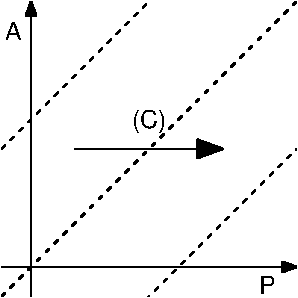
\includegraphics[height = 2cm]{../fig/APc.pdf} &
  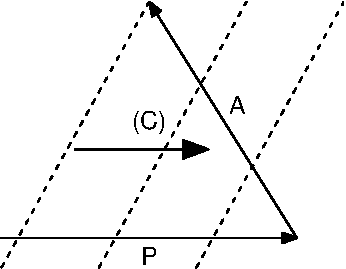
\includegraphics[height = 2cm]{../fig/APc_iso.pdf}  \\
  \midrule
  %%%% AC
  $$\begin{aligned}
    &AC(P) \\
    &P = C + A
  \end{aligned}$$ &
  The $AC(P)$ temporal plane is equivalent to the Lexis diagram only that birth cohort is given and period is embedded instead of the other way round. &
  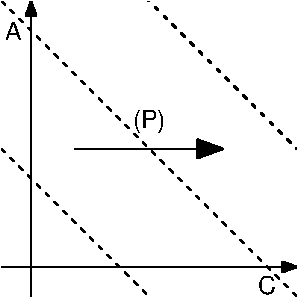
\includegraphics[height = 2cm]{../fig/ACp.pdf} &
  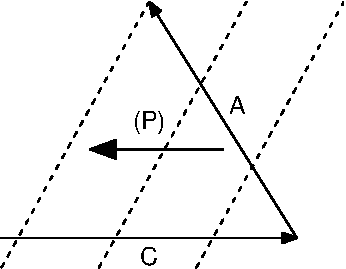
\includegraphics[height = 2cm]{../fig/ACp_iso.pdf}  \\
  \midrule
  %%%% CP
  $$\begin{aligned}
    &CP(A) \\
    &A = P - C
  \end{aligned}$$ &
  The $CP(A)$ temporal plane is equivalent to the Lexis diagram only that birth cohort is given and age is embedded instead of the other way round. &
  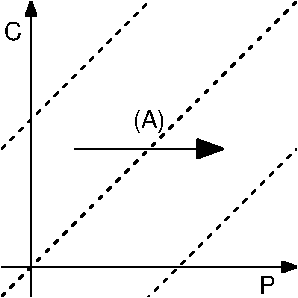
\includegraphics[height = 2cm]{../fig/CPa.pdf} &
  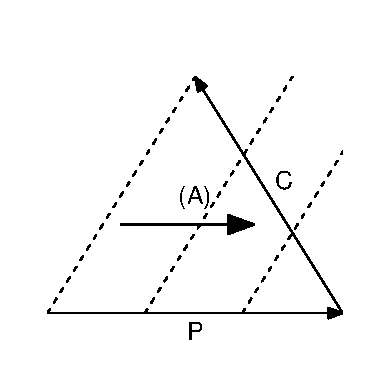
\includegraphics[height = 2cm]{../fig/CPa_iso.pdf}  \\
  \midrule
  %%%%%%%%%%%%%%%%%%%%%%%%%%%%%%%%%%%%%%%%%%%%%%%%%%%%%%%%%%%%%%%%%%%%%%%%%%%%%
  \multicolumn{4}{c}{\textsc{2-D Combinations of Thanatological Scales}} \\
  \midrule
  %%%% LD
  $$\begin{aligned}
    &LD(C) \\
    &C = D - L
  \end{aligned}$$ &
  foo. &
  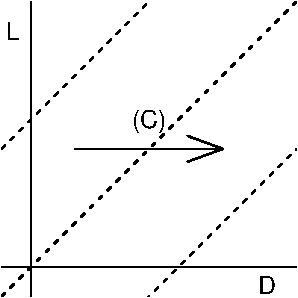
\includegraphics[height = 2cm]{../fig/LDc.pdf} &
  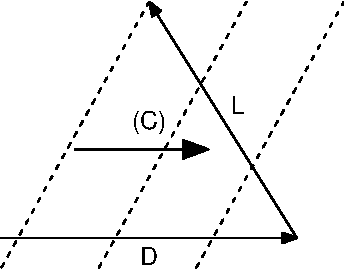
\includegraphics[height = 2cm]{../fig/LDc_iso.pdf}  \\
  \midrule
  %%%% TL
  $$\begin{aligned}
    &TL(A) \\
    &A = L - T
  \end{aligned}$$ &
  foo. &
  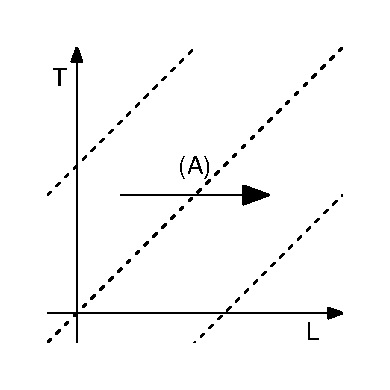
\includegraphics[height = 2cm]{../fig/TLa.pdf} &
  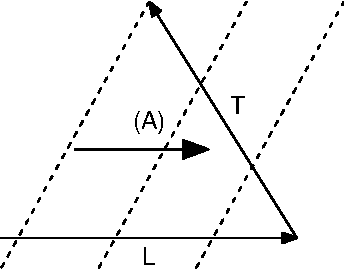
\includegraphics[height = 2cm]{../fig/TLa_iso.pdf}  \\
  \midrule
  %%%% TD
  $$\begin{aligned}
    &TD(P) \\
    &P = D - T
  \end{aligned}$$ &
  foo. &
  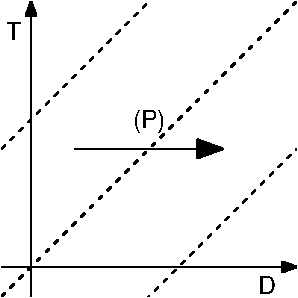
\includegraphics[height = 2cm]{../fig/TDp.pdf} &
  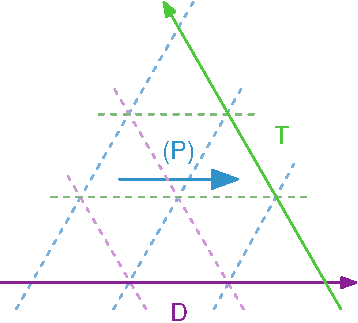
\includegraphics[height = 2cm]{../fig/TDp_iso.pdf}  \\
  \midrule
  %%%%%%%%%%%%%%%%%%%%%%%%%%%%%%%%%%%%%%%%%%%%%%%%%%%%%%%%%%%%%%%%%%%%%%%%%%%%%
  \multicolumn{4}{c}{\textsc{2-D Combinations of Lexis Scales and Thanatological Scales}} \\
  \midrule
  %%%% AL
  $$\begin{aligned}
    &AL(T) \\
    &T = A - L
  \end{aligned}$$ &
  foo. &
  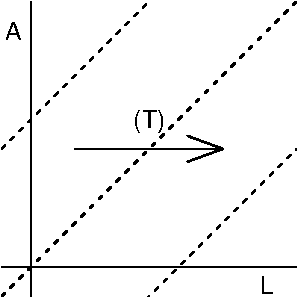
\includegraphics[height = 2cm]{../fig/ALt.pdf} &
  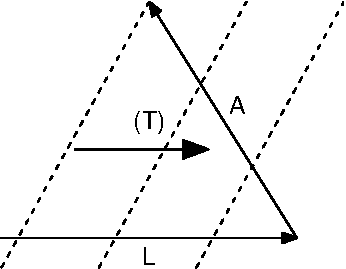
\includegraphics[height = 2cm]{../fig/ALt_iso.pdf}  \\
  \midrule
  %%%% LP
  $LP(-)$ &
  The $LP$ plane is \emph{non-informative}. No additional dimensions can be derived knowing just lifespan and period. &
  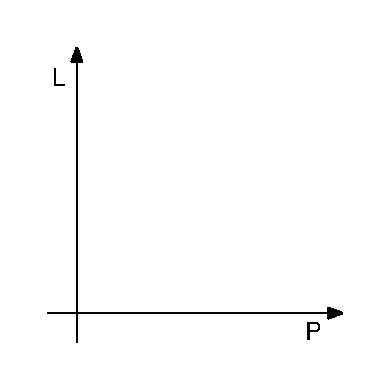
\includegraphics[height = 2cm]{../fig/LP.pdf} &
  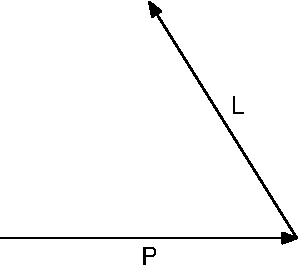
\includegraphics[height = 2cm]{../fig/LP_iso.pdf}  \\
  \midrule
  %%%% PD
  $$\begin{aligned}
    &PD(T) \\
    &T = D - P
  \end{aligned}$$ &
  foo. &
  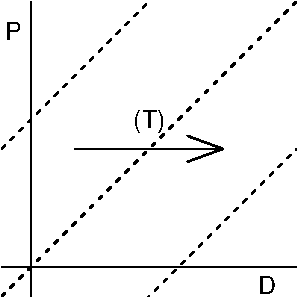
\includegraphics[height = 2cm]{../fig/PDt.pdf} &
  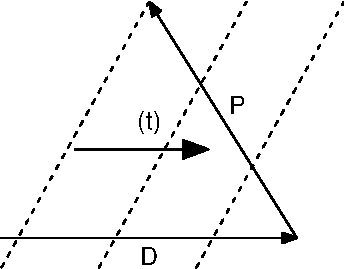
\includegraphics[height = 2cm]{../fig/PDt_iso.pdf}  \\
  \midrule
  %%%% CD
  $$\begin{aligned}
    &CD(L) \\
    &L = D - C
  \end{aligned}$$ &
  foo. &
  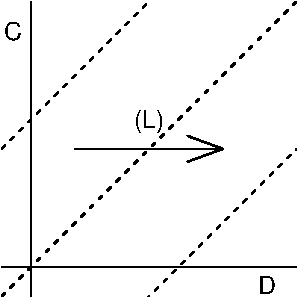
\includegraphics[height = 2cm]{../fig/CDl.pdf} &
  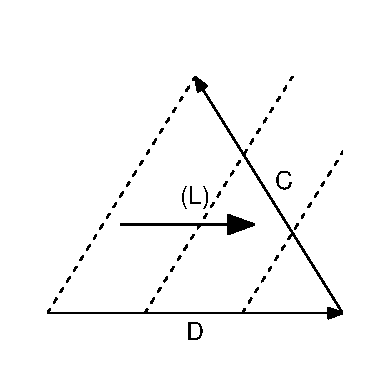
\includegraphics[height = 2cm]{../fig/CDl_iso.pdf}  \\
  \midrule
  %%%% CT
  $CT(-)$ &
  The $CT$ plane is \emph{non-informative}. No additional dimensions can be derived knowing just cohort and thanatological age. &
  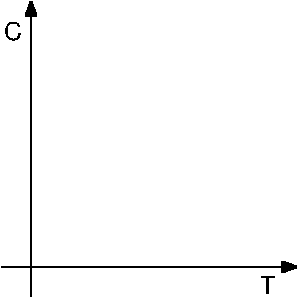
\includegraphics[height = 2cm]{../fig/CT.pdf} &
  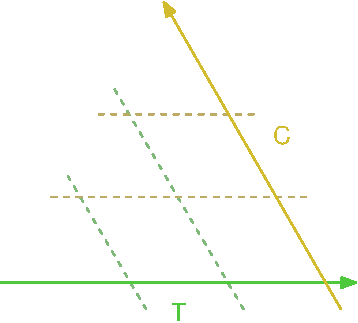
\includegraphics[height = 2cm]{../fig/CT_iso.pdf}  \\
  \midrule
  %%%% TA
  $$\begin{aligned}
    &TA(L) \\
    &L = T + A
  \end{aligned}$$ &
  The time already lived and the time still left sum up to the total lifespan. &
  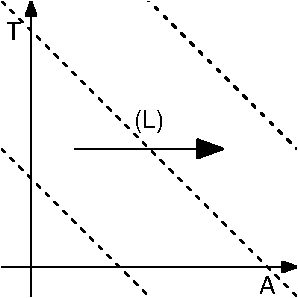
\includegraphics[height = 2cm]{../fig/TAl.pdf} &
  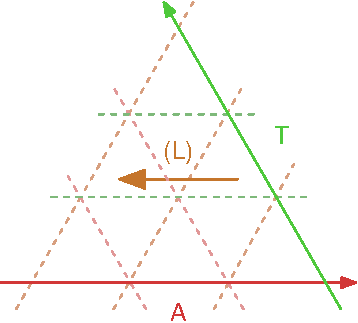
\includegraphics[height = 2cm]{../fig/TAl_iso.pdf}  \\
  \midrule
  %%%% AD
  $AD(-)$ &
  The $AD$ plane is \emph{non-informative}. No additional dimensions can be derived knowing just death cohort and age. &
  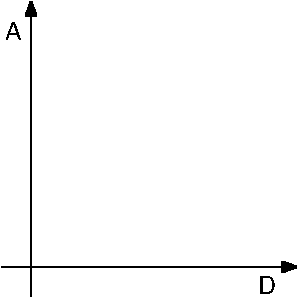
\includegraphics[height = 2cm]{../fig/AD.pdf} &
  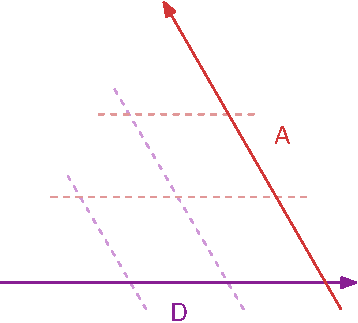
\includegraphics[height = 2cm]{../fig/AD_iso.pdf}  \\
  \midrule
  %%%% LC
  $$\begin{aligned}
    &LC(D) \\
    &D = C + L
  \end{aligned}$$ &
  foo. &
  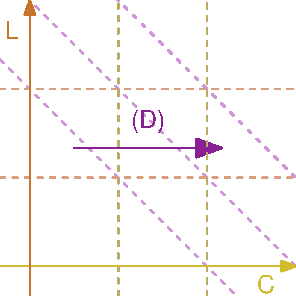
\includegraphics[height = 2cm]{../fig/LCd.pdf} &
  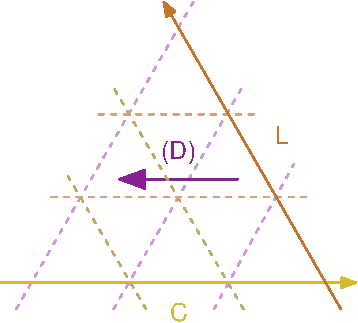
\includegraphics[height = 2cm]{../fig/LCd_iso.pdf}  \\
  \midrule
  %%%% TP
  $TP(D)$ &
  foo. &
  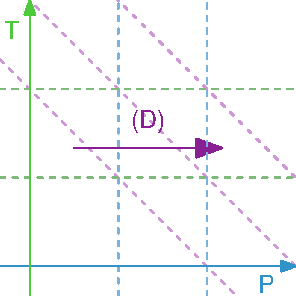
\includegraphics[height = 2cm]{../fig/TPd.pdf} &
  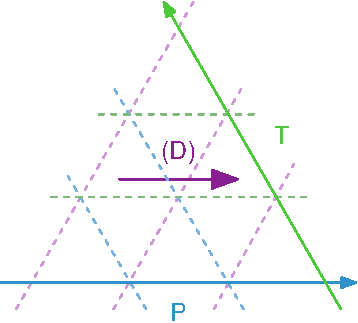
\includegraphics[height = 2cm]{../fig/TPd_iso.pdf}  \\
  \bottomrule
  \end{longtable}
\end{center}

\clearpage

\end{document}